\documentclass[14pt]{extarticle}
\usepackage[utf8]{inputenc}
\usepackage{tkz-euclide}
\usepackage{tikz} 
\usepackage{pdflscape}
\usepackage[margin=2cm]{geometry}
\usepackage{amsmath}

\begin{document}
\begin{center}
    \LARGE{\textbf{Esercitazione geometria Teorema Pitagora 2 - 07/10/2022 - 3B}}
\end{center}
\vspace{1cm}

%----- FINE CONSEGNA -----
\textbf{Problema 1:} Nel trapezio isoscele in figura la base minore, la base maggiore e l'altezza misurano: \(27cm\), \(37cm\) e \(12cm\). Calcola il perimetro, l'area e i lati obliqui.


\vspace{0.5cm}
\begin{tikzpicture}[scale=1, rotate=70]
    \tkzDefPoints{0/0/A,4/0/B,3/2/C,1/2/D}
    \tkzDrawPolygon(A,...,D)
    \tkzDrawPoints(A,...,D)
    \tkzDefMidPoint(B,C)
    \tkzDefPointBy[projection=onto B--A](C) \tkzGetPoint{H} %ALTEZZA
    \tkzDrawSegments[style=dashed](C,H)
    \tkzLabelPoints[left](D)
    \tkzLabelPoints[below](A)
    \tkzLabelPoints[above](C)
    \tkzLabelPoints[above](B)
    \tkzLabelPoints[right](H)
\end{tikzpicture}

\vspace{0.5cm}
\textbf{Problema 2:} Nel triangolo isoscele l'area misura \(75cm^2\) e il lato \(\overline{CB}\) misura \(15cm\). Calcola la misura delle tre altezze del triangolo.\vspace{0.5cm}\\
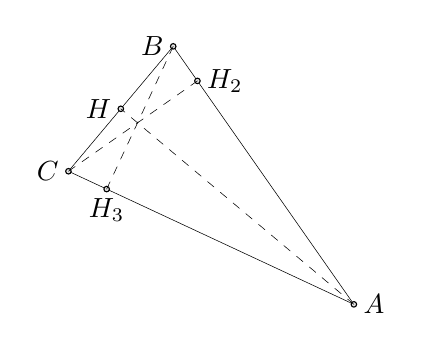
\begin{tikzpicture}[rotate=125]
    \tkzDefPoint(2,3){A}
    \tkzDefShiftPoint[A](0:4){B}
    \tkzDefShiftPoint[A](30:4){C}
    \tkzDefMidPoint(B,C)
    \tkzGetPoint{H}
    \tkzDefMidPoint(B,A)
    \tkzGetPoint{H_2}
    \tkzDefMidPoint(A,C)
    \tkzGetPoint{H_3}
    \tkzDrawSegments(A,B B,C C,A)
    %\tkzMarkSegments[mark=|](A,B A,C)
    \tkzDefPointBy[projection=onto B--A](C) \tkzGetPoint{H_2}
    \tkzDefPointBy[projection=onto A--C](B) \tkzGetPoint{H_3}
    \tkzDrawPoints(A,B,C,H, H_2, H_3)
    \tkzLabelPoints[left](B,C, H)
    \tkzLabelPoints[right](A)
    \tkzLabelPoints[right](H_2)
    \tkzLabelPoints[below](H_3)
    \tkzDrawSegments[style=dashed](A,H C,H_2 B,H_3)
\end{tikzpicture}

\vspace{0.5cm}
\textbf{Problema 3:} La figura ha un'area di \(864cm^2\) e il lato di \(30cm\). Calcola la misura di \(\overline{CH}\) e la misura dei segmenti \(\overline{BH}\) e \(\overline{AH}\).\\
%rombo
\hspace{0.5cm}
\begin{tikzpicture}[scale=1, rotate=0]
    \tkzDefPoints{2/0/A,4/1/D,0/1/B,2/2/C,2/1/O}
    \tkzDrawPolygon(A,...,D)
    \tkzDrawPoints(A,...,D)
    \tkzDefPointBy[projection=onto B--A](C) \tkzGetPoint{H}
    \tkzLabelPoints[below](A,H)
    \tkzMarkRightAngle(C,H,B) % segno perpendicolarità 90°
    \tkzLabelPoints[right](D)
    \tkzLabelPoints[left](B)
    \tkzLabelPoints[above](C)
    \tkzDrawSegments[style=dashed](C,H)
    %\tkzLabelPoints[below right](O)
    %\tkzDrawSegments(A,C)
    %\tkzDrawSegments(B,D)
\end{tikzpicture}

\clearpage
\textbf{Problema 4:} nel rettangolo il perimetro e la base misurano \(68cm\) e \(24cm\). Calcola altezza, diagonale e area.\\

\vspace{0.5cm}
%quadrato
\hspace{0.5cm}
\begin{tikzpicture}[scale=1, rotate=105]
    \tkzDefPoints{0/0/A,2/0/B,2/4/C,0/4/D}
    \tkzDrawPolygon(A,...,D)
    \tkzDrawPoints(A,...,D)
    \tkzLabelPoints[right](A)
    \tkzLabelPoints[below](D)
    \tkzLabelPoints[above](B)
    \tkzLabelPoints[above left](C)
    \tkzDrawSegments[style=dashed](A,C)
\end{tikzpicture}

\vspace{1cm}
\textbf{Problema 5:} nel trapezio rettangolo l'altezza e la base minore misurano \(24cm\) e \(25cm\), mentre il lato obliquo \(25cm\). Calcola e disegna la diagonale maggiore, calcola perimetro e area.\\

\vspace{0.5cm}
\begin{tikzpicture}[scale=1, rotate=42]
    \tkzDefPoints{0/0/A,4/0/B,3/2/C,0/2/D}
    \tkzDrawPolygon(A,...,D)
    \tkzDrawPoints(A,...,D)
    \tkzDefMidPoint(B,C)
    \tkzDefPointBy[projection=onto B--A](C) \tkzGetPoint{H} %ALTEZZA
    \tkzDrawSegments[style=dashed](C,H)
    \tkzLabelPoints[left](D)
    \tkzLabelPoints[below](A)
    \tkzLabelPoints[above](C)
    \tkzLabelPoints[right](B)
    \tkzLabelPoints[below right](H)
\end{tikzpicture}

\vspace{1cm}
\textbf{Problema 6:} il parallelogramma è diviso dalla diagonale minore \(\overline{DB}\) in due triangoli rettangoli. La diagonale minore misura \(48cm\) ed il lato ad essa perpendicolare misura \(36cm\). Calcola il perimetro e area.

\vspace{0.5cm}
\begin{tikzpicture}[scale=1.1]
    %initialisation
    %\tkzInit[xmin=0,xmax=4,ymin=0,ymax=2] 
    %\tkzClip[space=.5] 
    %definitions
    \tkzDefPoint(0,0){A} 
    \tkzDefPoint(5,0){B} 
    \tkzDefPoint(6,2){C} 
    \tkzDefPoint(1,0){H}
    \tkzDefPointWith[colinear= at C](B,A) \tkzGetPoint{D}
    %drawing
    \tkzDrawPolygon(A,B,C,D)
    %\tkzDrawSegments[blue,dashed](A,C B,D)
    %label
    \tkzLabelPoints[below](A,B)
    \tkzLabelPoints[above](C,D)
    \tkzDrawSegments[style=dashed](D,B)
    \tkzMarkRightAngle(D,B,C)
    \tkzMarkRightAngle(B,D,A)
    %\tkzLabelSegment[above,pos=.7,sloped](A,C){$x+y$}
    %\tkzLabelSegme
\end{tikzpicture}
\clearpage

\end{document}


